\documentclass{physics_notes}

\usepackage{makeidx}
\usepackage{showidx}

\title{Complex Analysis}
%\author{St Aidan's Physics Society}
\date{\today}
\usetikzlibrary{decorations}
\usetikzlibrary{decorations.pathmorphing}
\usetikzlibrary{decorations.markings}
\usetikzlibrary{calc}

\makeindex

\begin{document}

\maketitle
\tableofcontents
\newpage

\section*{Introduction}

These notes are based on the Complex Analysis course delivered in Michaelmas 2019, by Prof Ruth Gregory. 

There are also frequent references, both explicit and otherwise, made to the book \emph{Mathematical Methods for Physics and Engineering} by K. F. Riley, M. P. Hobson, and S. J. Bence. Relevant chapters of the book are highlighted using coloured square brackets, e.g. \book{24.5}.

Contributors: Ben Amies-King

\section{The $\mathbb{C}$ plane}
\subsection{Complex numbers}

\index{complex numbers}
A simple motivation for studying complex numbers can be gained by considering the roots of a quadratic of negative determinant, such as:

\begin{equation}\label{eq:complex_quad}
x^2 -2x + 2 = 0
\end{equation}

which has roots:

\begin{align}
x &= \frac{2 \pm 2\sqrt{-1}}{2} \nonumber \\
&= 1 \pm i \nonumber
\end{align}

where we denote $\sqrt{-1}$ with $i$. This is the conventional representation of a complex number:

\begin{equation}
z = x + iy = \Re\{z\} + i\Im\{z\}
\end{equation}

We can also express $z$ as coordinates on an Argand diagram, $z = (x,y)$. The roots of Equation \ref{eq:complex_quad} are shown in this form in Figure \ref{fig:argand_quad}.
\index{Argand diagram}

\begin{figure}[h]
\centering
\begin{tikzpicture}
    \begin{scope}[thick,font=\scriptsize]
    % Axes:
    % Are simply drawn using line with the `->` option to make them arrows:
    % The main labels of the axes can be places using `node`s:
    \draw [->] (-2,0) -- (2,0) node [above]  {$\Re\{z\}$};
    \draw [->] (0,-2) -- (0,2) node [left] {$\Im\{z\}$};

    % Points
    \draw (1,1) circle[radius=1pt];
    \draw (1,-1) circle[radius=1pt];

    % Axes labels:
    \draw (1,-3pt) -- (1,3pt)   node [above] {$1$};
    \draw (-1,-3pt) -- (-1,3pt) node [above] {$-1$};
    \draw (-3pt,1) -- (3pt,1)   node [right] {$i$};
    \draw (-3pt,-1) -- (3pt,-1) node [right] {$-i$};

    \end{scope}
\end{tikzpicture}
\caption{The complex numbers $z = 1 \pm i$ represented on an Argand diagram. }\label{fig:argand_quad}
\end{figure}

We define the modulus and argument of the complex number $z = x + iy$:

\begin{align*}
|z| &= \sqrt{x^2 + y^2} \\ \\
arg\{z\} &= \tan^{-1}{\frac{y}{x}}
\end{align*}

This leads into an alternative expression of complex numbers known as the polar representation:

\begin{align*}
z = x + iy \longrightarrow z = r e^{i\theta}; \; r  = |z|, \, \theta = arg\{z\}
\end{align*}

We must also define the complex conjugate $z^{\star}$ of $z$, given by:

\[ z^{\star} = x - iy = \Re\{z\} - i\Im\{z\} \]

which implies:

\begin{align*} 
\Re\{z^\star\} &= \Re\{z\}\\ 
\Im\{z^\star\} &= -\Im\{z\} \\ 
|z^\star| &= |z| \\ 
arg\{z^\star\} &= -arg\{z\} 
\end{align*}

We can then deduce:

\begin{equation}
\Re\{z\} = \frac{z + z^\star}{2} 
\end{equation}
\begin{equation}
\Im\{z\} = \frac{z - z^\star}{2}
\end{equation}

The behaviour of complex numbers under simple manipulations (addition, multiplication, exponentiation etc.) can be determined from the polar expression, and so we won't go into it here. 

\subsection{Complex functions}

\index{complex functions}
We can define a complex function $f$:

\begin{align*}
f: \; \mathbb{C} &\rightarrow \mathbb{C} \\
z &\rightarrow f(z) = u(x, y) + iv(x, y)
\end{align*}

where $u, v$ are real functions of real variables $x, y$. For example:

\begin{enumerate}
\item{Polynomials, $f(z) = z^2$ \begin{align*} f(x + iy) &= (x + iy)^2 \\ &= x^2 + 2ixy - y^2 \\ &= x^2 - y^2 + i2xy\end{align*} \\ So $u(x, y) = x^2 - y^2, \, v(x, y) = 2xy$}
\item{Fractional exponents, $f(z) = \sqrt{z}$ \begin{align*} f(re^{i\theta}) &= \sqrt{re^{i\theta}} \\ &= \sqrt{r} e^{\frac{i\theta}{2}}\end{align*} \\ So $u = \sqrt{r}\cos{\frac{\theta}{2}}, \, v = \sqrt{r}\sin{\frac{\theta}{2}}$}
\end{enumerate}

We haven't explicitly specified a range for $\theta$, however it is clear that we will need at least $\theta \in \left[0, 2\pi\right]$ in order to define contours over the whole complex plane. We must then consider multivaluedness of certain functions, as it this will otherwise pose problems when we come to consider concepts such as integration. 

From above, when $f(z) = \sqrt{z}$:

\begin{equation*}
f(re^{i\theta}) = \sqrt{r} e^{\frac{i\theta}{2}}
\end{equation*}

We can clearly see that adding $2\pi n$ to the argument of a complex number $z = re^{i\theta}$ returns the same complex number:

\[re^{i(\theta + 2\pi n)} = re^{i\theta}\cdot e^{i 2\pi n} = re^{i\theta}\cdot 1^n = re^{i\theta} \]

However, putting $re^{i(\theta + 2\pi n)}$ into $f(z) = \sqrt{z}$ produces a concerning result:

\begin{align*}
f(re^{i(\theta + 2\pi n)}) &= \sqrt{r} e^{\frac{i(\theta + 2\pi n)}{2}} \\
&= \sqrt{r} e^{\frac{i\theta}{2}}\cdot e^{i \pi n} \\
&= \sqrt{r} e^{\frac{i\theta}{2}}\cdot (-1)^n 
\end{align*}

So for odd $n$, we have that $f(z) = -\sqrt{z}$. Traversing any closed contour results in a change of sign of $f(z)$: it switches to a different branch when crossing the real axis. Now consider $f(z) = \ln{z}$:

\begin{align*}
f(re^{i(\theta + 2\pi n)}) &= \ln{re^{i\theta + 2\pi n}} \\
&= \ln{r} + \ln{e^{i\theta}} + \ln{e^{i 2\pi n}} \\
&= \ln{r} + i(\theta + 2\pi n)
\end{align*}

Hence every full contour traversal, $f(z)$ changes value and never returns to its original. This multivaluedness defies a key property called analyticity, which we will cover later, so we need a solution to force functions to become single valued. 

\subsubsection*{Branch points and branch cuts \book{24.5}}
\index{branch points}
\index{branch cuts}

In the case of $f(z = \sqrt{z}$, we can see that any contour that traverses the real axis only once must contain the origin (and this is unique the origin in this case), and so  we call the origin a \emph{branch point}. We construct a corresponding \emph{branch cut} from the origin to infinity (in any direction, however generally along the real axis). This branch cut is an impassable barrier from the perspective of any contour, and so we are forcing $f(z)$ to be single valued. 

\begin{figure}
\centering
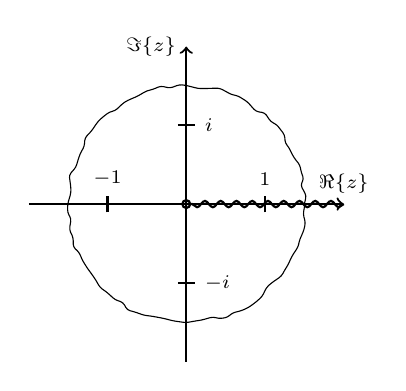
\begin{tikzpicture}
\begin{scope}[thick,font=\scriptsize]
    % Axes:
    % Are simply drawn using line with the `->` option to make them arrows:
    % The main labels of the axes can be places using `node`s:
    \draw [->] (-2,0) -- (2,0) node [above]  {$\Re\{z\}$};
    \draw [->] (0,-2) -- (0,2) node [left] {$\Im\{z\}$};

    % Points
    \draw [decorate,decoration={snake,amplitude=.4mm,segment length=2mm}] (2,0) -- (0,0) node [draw=black, circle, fill=none, inner sep=1pt, pos=1, label] {};


    % Axes labels:
    \draw (1,-3pt) -- (1,3pt)   node [above] {$1$};
    \draw (-1,-3pt) -- (-1,3pt) node [above] {$-1$};
    \draw (-3pt,1) -- (3pt,1)   node [right] {$i$};
    \draw (-3pt,-1) -- (3pt,-1) node [right] {$-i$};
    \end{scope}
	\begin{scope}[decoration={random steps,segment length=3pt,amplitude=1pt}]
        \draw[decorate,rounded corners=1pt] (0,0) ellipse (1.5cm and 1.5cm);
    \end{scope}
\end{tikzpicture}
\caption{A contour around a branch point at $z = 0$, with a branch cut along the positive real axis.}
\end{figure}

\begin{example}{Finding branch cuts}
Let $f(z) = \sqrt{z^4 + 1}$. We know branch points occur when $z^4 + 1 = 0 \iff z^4 = -1$, so we have branch points:

\[ z = e^\frac{i\pi}{4},\; e^\frac{3i\pi}{4},\; e^\frac{5i\pi}{4},\; e^\frac{7i\pi}{4} \]

for $\theta \in \left[0, 2\pi\right]$. We can then construct branch cuts in a number of ways (see Figure \ref{fig:ex_branch_cuts})

\begin{figure}
	\centering
	\begin{subfigure}{.4\linewidth}
		\centering
		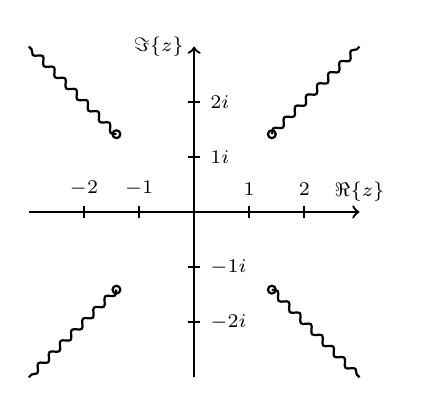
\begin{tikzpicture}[scale=0.7]
		    \begin{scope}[thick,font=\scriptsize]
		    % Axes:
		    % Are simply drawn using line with the `->` option to make them arrows:
		    % The main labels of the axes can be places using `node`s:
		    \draw [->] (-3,0) -- (3,0) node [above]  {$\Re\{z\}$};
		    \draw [->] (0,-3) -- (0,3) node [left] {$\Im\{z\}$};

		    % Points
    		\draw [decorate,decoration={snake,amplitude=.4mm,segment length=2mm}] (1.41,1.41) -- (3,3) node [draw=black, circle, fill=none, inner sep=1pt, pos=0] {};
    		\draw [decorate,decoration={snake,amplitude=.4mm,segment length=2mm}] (1.41,-1.41) -- (3,-3) node [draw=black, circle, fill=none, inner sep=1pt, pos=0] {};
    		\draw [decorate,decoration={snake,amplitude=.4mm,segment length=2mm}] (-1.41,1.41) -- (-3,3) node [draw=black, circle, fill=none, inner sep=1pt, pos=0] {};
    		\draw [decorate,decoration={snake,amplitude=.4mm,segment length=2mm}] (-1.41,-1.41) -- (-3,-3) node [draw=black, circle, fill=none, inner sep=1pt, pos=0] {};

		    % Axes labels:
		    % Are drawn using small lines and labeled with `node`s. The placement can be set using options
		    \iffalse% Single
		    % If you only want a single label per axis side:
		    \draw (1,-3pt) -- (1,3pt)   node [above] {$1$};
		    \draw (-1,-3pt) -- (-1,3pt) node [above] {$-1$};
		    \draw (-3pt,1) -- (3pt,1)   node [right] {$i$};
		    \draw (-3pt,-1) -- (3pt,-1) node [right] {$-i$};
		    \else% Multiple
		    % If you want labels at every unit step:
		    \foreach \n in {-2,...,-1,1,2,...,2}{%
		        \draw (\n,-3pt) -- (\n,3pt)   node [above] {$\n$};
		        \draw (-3pt,\n) -- (3pt,\n)   node [right] {$\n i$};
		    }
		    \fi
		    \end{scope}
		\end{tikzpicture}
		\caption{The complex numbers $z = 1 \pm i$ represented on an Argand diagram. }
	\end{subfigure}\hspace{1cm}%
	\begin{subfigure}{.4\linewidth}
		\centering
		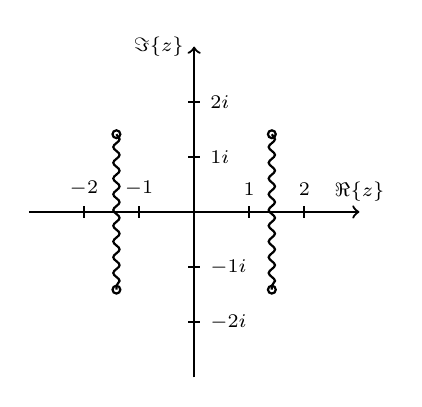
\begin{tikzpicture}[scale=0.7]
		    \begin{scope}[thick,font=\scriptsize]
		    % Axes:
		    % Are simply drawn using line with the `->` option to make them arrows:
		    % The main labels of the axes can be places using `node`s:
		    \draw [->] (-3,0) -- (3,0) node [above]  {$\Re\{z\}$};
		    \draw [->] (0,-3) -- (0,3) node [left] {$\Im\{z\}$};

		    % Points
    		\draw [decorate,decoration={snake,amplitude=.4mm,segment length=2mm}] (1.41,1.41) -- (1.41,-1.41) node [draw=black, circle, fill=none, inner sep=1pt, pos=1] {} node [draw=black, circle, fill=none, inner sep=1pt, pos=0] {};
    		\draw [decorate,decoration={snake,amplitude=.4mm,segment length=2mm}] (-1.41,1.41) -- (-1.41,-1.41) node [draw=black, circle, fill=none, inner sep=1pt, pos=1] {} node [draw=black, circle, fill=none, inner sep=1pt, pos=0] {};

		    % Axes labels:
		    % Are drawn using small lines and labeled with `node`s. The placement can be set using options
		    \iffalse% Single
		    % If you only want a single label per axis side:
		    \draw (1,-3pt) -- (1,3pt)   node [above] {$1$};
		    \draw (-1,-3pt) -- (-1,3pt) node [above] {$-1$};
		    \draw (-3pt,1) -- (3pt,1)   node [right] {$i$};
		    \draw (-3pt,-1) -- (3pt,-1) node [right] {$-i$};
		    \else% Multiple
		    % If you want labels at every unit step:
		    \foreach \n in {-2,...,-1,1,2,...,2}{%
		        \draw (\n,-3pt) -- (\n,3pt)   node [above] {$\n$};
		        \draw (-3pt,\n) -- (3pt,\n)   node [right] {$\n i$};
		    }
		    \fi
		    \end{scope}
		\end{tikzpicture}
		\caption{The complex numbers $z = 1 \pm i$ represented on an Argand diagram. }
	\end{subfigure}
	\caption{Two options for branch cuts for the function $f(z) = \sqrt{z^4 + 1}$.}
\end{figure}
\end{example}

\subsection{Logarithm and Exponential functions \book{24.4}}

We define:

\[\exp{z} = \sum_{n=0}^\infty \frac{z^n}{n!} \]

By showing that $\exp{z_1}\exp{z_2} = \exp{z_1 + z_2}$, we can see $\exp{z}$ reduces to $\exp{x}$ for $\Im\{z\} = 0$, and so complex exponentials behave the same as real exponentials. For $a > 0$ we can write:

\[ a^z = \exp{z\ln{a}} \]

and so putting $a = e$ shows that $e^z$ and $\exp{z}$ are interchangeable.

We have already seen that logarithms require branch cuts. As a further demonstration, consider:

\begin{align*}
\ln{6} &= \ln{(-2)(-3)} \\
&\stackrel{*}{=} \ln{2e^{i\pi}} + \ln{3e^{i\pi}} \\
&= \ln{2} + i\pi + \ln{3} + i\pi \\
&= \ln{6} + 2i\pi
\end{align*}

At the starred step. we have simply expressed $-2$ and $-3$ in polar form. The extra factor fo $2i\pi$ represents us changing to the wrong branch. By introducing a branch cut from $0$ to $-\infty$, we restrict $\arg{z} \in [-\pi,\pi]$ and can then choose:

Instead using $-2 = 2e^{i\pi}$, $-3 = 3e^{-i\pi}$ giving $6 = (-2)(-3) = 6e^{0} = 6$.

\subsection{Trigonometric and Hyperbolic functions}

As we have considered the extension of the exponential function, the extension of trigonometric and hyperbolic functions follows trivially:

\begin{align*}
\cos{\theta} = \frac{e^{i\theta} + e^{-i\theta}}{2} &\longrightarrow \cos{z} = \frac{e^{iz} + e^{-iz}}{2}\\
\sin{\theta} = \frac{e^{i\theta} + e^{-i\theta}}{2} &\longrightarrow \sin{z} = \frac{e^{iz} - e^{-iz}}{2i}\\
\cosh{\theta} = \frac{e^{\theta} + e^{-\theta}}{2} &\longrightarrow \cosh{z} = \frac{e^{z} + e^{-z}}{2}\\
\sinh{\theta} = \frac{e^{\theta} + e^{-\theta}}{2} &\longrightarrow \sinh{z} = \frac{e^{z} - e^{-z}}{2}
\end{align*}

We see:
\index{trigonometric functions}\index{hyperbolic functions}
\begin{align}
\cos{z} &= \cosh{iz} \\
\sin{z} &= i\sinh{iz} \\
\cosh{z} &= \cos{iz} \\
\sinh{z} &= i\sin{iz}
\end{align}

This shows that the hyperbolic functions are periodic in the imaginary plane, in the same way that the trigonometric functions are periodic in the real plane. 

\section{Differentiation and Cauchy-Riemann Equations}
\index{differentiation}
Recall $f'(x) = \lim_{h\to 0} \frac{f(x + h) - f(x)}{h}$. Before we can consider an extension of differentiation to the complex plane, we need to define a crucial property.

\subsection{Continuity}

A complex function $f(z)$ is called \emph{continuous} at $z$ when we have:

\[ \lim_{z\to z_0} f(z) = w \iff \forall \epsilon > 0 \exists \delta > 0 s.t. |z - z_0| < \delta \implies |f(z) - w] < \epsilon \]

This definition is the same in $\mathbb{C}$ as in $\mathbb{R}$, $\mathbb{R}^2$ etc. 

Note that for this definition to hold, we must have that $\lim_{z\to z_0} f(z)$ is path independent. 

We can now return to considering how to define differentiation.

\subsection{Differentiation \book{24.1}}

Despite the fact that we can think of complex numbers as 2 dimensional vectors, we can't import vector derivatives into the complex plane. This becomes clear when we consider the domains and codomains of grad ($\grad$), div ($\div$), and curl ($\curl$):

\begin{align*}
\grad: \mathbb{R} &\longrightarrow \mathbb{R}^n \\
&\\
\div: \mathbb{R}^n &\longrightarrow \mathbb{R} \\
&\\
\curl: \mathbb{R}^3 &\longrightarrow \mathbb{R}^3 
\end{align*}

We clearly require a complex derivative $\vec{\nabla}_{\mathbb{C}}$ such that:

\[ \vec{\nabla}_{\mathbb{C}}: \mathbb{C} \longrightarrow \mathbb{C} \]

We will try to extend the real definition of the derivative to the complex plane. Consider:

\[ \vec{\nabla}_{\mathbb{C}} f = \frac{df}{dz} = \lim_{\delta\to 0} \frac{f(z+\delta) - f(z)}{\delta} \hspace{1in} \delta \in \mathbb{C}\]

In order to justify this definition, we will try some basic functions. 

Consider $f(z) = z$:

\begin{align*}
\frac{df}{dz} = \lim_{\delta\to 0} \frac{\cancel{z}+\delta - \cancel{z}}{\delta} = 1
\end{align*}

 \begin{align*}
\frac{df}{dz} &= \lim_{\delta\to 0} \frac{(z+\delta)^2 - z^2}{\delta} \\
&= \lim_{\delta\to 0} \frac{2\delta z - \delta^2}{\delta} \\
&= 2z
\end{align*}

Both of the above give the expected result. Now consider $f(z) = z^\star$:

\begin{align*}
\frac{df}{dz} &= \lim_{\delta\to 0} \frac{(z+\delta)^\star - z^2}{\delta} \\
&= \frac{\delta^\star}{\delta} 
\end{align*}

If $\delta = |\delta|e^{i\theta}$ then $\frac{\delta^\star}{\delta} = e^{-2i\theta}$, so the limit is not well-defined, hence $f(z) = z^\star$ is not differentiable. Finally, consider $f(z) = |z|^2 = z z^\star$:

\begin{align*}
\frac{df}{dz} &= \lim_{\delta\to 0} \frac{(z+\delta) (z+\delta)^\star - z z^\star}{\delta} \\
&= \frac{\delta z^\star + \delta^\star z + \delta \delta^\star}{\delta} \\
&= z^\star + z\frac{\delta^*}{\delta} + \mathcal{O}(\delta^2)
\end{align*}

So $f(z) = |z|^2$ is only differentiable at $z=0$, as $z\frac{\delta^*}{\delta}$ is only path-independent at $z=0$. This uncertainty in whether functions can be differentiated motivates us to introduce a new property of functions.

\subsection{Analytic Functions}
\index{analytic functions}
\index{neighbourhood}
Firstly, we define a neighbourhood of $z\in \mathbb{C}$ as an open set $U$ such that $z \in U$.

We can then say that $f: \mathbb{C} \leftarrow \mathbb{C}$ is analytic (or equivalently holomorphic) at $z_0 \in \mathbb{C}$ if $\exists$ a neighbourhood $U$ of $z_0$ on which $f$ is differentiable at all points in $U$.

Note that whilst $|z|^2$ is differentiable at $z = 0$, it is not analytic as it isn't differentiable in an arbitrarily small neighbourhood around $z=0$.

If a function $f$ is analytic on the neighbourhood $U = \mathbb{C}$, then it is called an \emph{entire} function.

\subsection{Cauchy-Riemann Equations \book{24.2}}
\index{Cauchy-Riemann equations}
\index{differentiation}
We will now examine complex differentiation more rigorously. Consider $f(x + iy) = u(x,y) + iv(x,y)$. Then:

\begin{align*}
\frac{f(z) - f(z_0)}{z-z_0} &= \frac{u(x_0 + \delta x, y_0 + \delta y) -u(x_0, y_0)}{\delta x + i\delta y} + \frac{iv(x_0 + \delta x, y_0 + \delta y) - iv(x_0,y_0)}{\delta x + i\delta y} \\
&= \frac{\delta x \frac{\partial u}{\partial x} + \delta y \frac{\partial u}{\partial y}}{\delta x + i\delta y} + \frac{i \left(\delta x \frac{\partial v}{\partial x} + \delta y \frac{\partial v}{\partial y} \right)}{\delta x + i\delta y} + \mathcal{O}(\delta^2) \\
&= \frac{\delta x \left(\frac{\partial u}{\partial x} + i\frac{\partial v}{\partial x}\right) + i\delta y \left(-i\frac{\partial u}{\partial y} + \frac{\partial v}{\partial y}\right)}{\delta x _ i\delta y}
\end{align*}

In order to cancel the denominator and have $\lim_{z\to z_0} \frac{f(z) - f(z_0)}{z-z_0}$ exist, we require:

\[ \frac{\partial u}{\partial x} + i\frac{\partial v}{\partial x} = -i\frac{\partial u}{\partial y} + \frac{\partial v}{\partial y} \]

Equivalently:

\begin{align*}
\frac{\partial u}{\partial x} &= \frac{\partial v}{\partial y} \\
\frac{\partial v}{\partial x} &= -\frac{\partial u}{\partial y}
\end{align*}

Once again, consider: 

\[ f(z) = z^2 = (x + iy)^2 = x^2 - y^2 + 2ixy \]

So:

\begin{align*}
u &= x^2 - y^2 :  & \frac{\partial u}{\partial x} = 2x \hspace{1cm} & \frac{\partial u}{\partial y} = -2y \\
v &= 2xy : & \frac{\partial v}{\partial x} = 2y \hspace{1cm} & \frac{\partial v}{\partial y} = 2x 
\end{align*}

So we have $\frac{\partial u}{\partial x} = \frac{\partial v}{\partial y}$, $\frac{\partial v}{\partial x} = -\frac{\partial u}{\partial y}$ so $f(z) = z^2$ is \emph{entire}, as we didn't place any restrictions on $z_0$ at the start of the process. 

Note that these equalities imply $u$ obeys a Laplace equation:
\index{Laplace equation}
\begin{align*}
\frac{\partial^2 u}{\partial x^2} &= \frac{\partial}{\partial x}\frac{\partial u}{\partial x} = \frac{\partial}{\partial x} \frac{\partial v}{\partial y} = \frac{\partial^2 v}{\partial x \partial y} = \frac{\partial}{\partial y}\frac{\partial v}{\partial x} = -\frac{\partial}{\partial y}\frac{\partial u}{\partial y} = -\frac{\partial^2 u}{\partial y^2} \\
&\implies \frac{\partial^2 u}{\partial x^2} + \frac{\partial^2 u}{\partial y^2} = 0
\end{align*}

Suppose we consider $z$ and $z^\star$ to be independent functions. We can write:

\[ x = \frac{z + z^\star}{2}, \; y = \frac{z - z^\star}{2i} \]

Then 

\begin{align*} 
\frac{\partial}{\partial z^\star} &= \frac{\partial x}{\partial z^\star}\frac{\partial}{\partial x} + \frac{\partial y}{\partial z^\star}\frac{\partial}{\partial y}\\
&= \frac{1}{2}\left(\frac{\partial}{\partial x} + i\frac{\partial}{\partial y} \right)
\end{align*}

Giving:

\[ \frac{\partial f}{\partial z^\star} = \frac{1}{2}\left(\frac{\partial u}{\partial x} + i\frac{\partial u}{\partial y} + i\frac{\partial v}{\partial x} - \frac{\partial v}{\partial y}\right) = 0 \]

if and only if the Cauchy-Riemann equations hold. Hence $\frac{\partial f}{\partial z^\star} = 0$ forms a compact test for analyticity. 
\index{analytic functions}

\section{Complex Integration and Cauchy's Theorem}
\index{integration}

\subsection{Subsets of $\mathbb{C}$ plane}

A continuous curve, $\gamma$, on $\mathbb{C}$ is a map from the reals onto $\mathbb{C}$:

\begin{equation*}
\gamma : \left[a,b\right] \subset \mathbb{R} \longrightarrow \mathbb{C}
\end{equation*}

with $\gamma (a)$ the initial point and $\gamma (b)$ the final point. $-\gamma$ is the same path, but in the opposite direction.

An open set $G$ is said to be split if 

\begin{equation*}
G = G_1 \cup G_2 \hspace{.5cm} \text{with} \hspace{.5cm} G_1 \cap G_2 = \{\phi\}; \hspace{.2cm} G_1 , G_2 \neq \{\phi\}
\end{equation*}

G is connected if it does not split; this is equivalent to the existence of a curve $\gamma \subset G$ linking any pair of points in $G$.

$G$ is called \emph{simply connected} if any pair of lines connecting two points in $G$ can be deformed into eachother without leaving $G$.

\subsection{Complex Integration \book{24.8}}
\index{integration}

For integration on $\mathbb{R}$, there is no ambiguity in the path between two points however on $\mathbb{C}$ we can choose many curves between two points, and so we must specify one. We can do this via a parameterisation:

\begin{equation*}
\gamma : \hspace{.2cm} \zeta (t) = x(t) + i y(t) \implies d\zeta = dx + i dy = (x' + i y')dt
\end{equation*}

So we can express a general integration:

\begin{align*}
\int_{\gamma} f(z) dz &= \int_{\gamma} (u + iv)(dx + idy) \\
&= \int_\gamma [(udx - vdy) + i(vdx + udy)]
\end{align*}

\begin{example}{$\int_\gamma z^2 dz$ for $\gamma: [0,\pi] \rightarrow \mathbb{C}$, $t \leftarrow e^{it}$}

We thus have the parameterisation $x = \cos{t} \hspace{.2cm} y = \sin{t}$.
\index{parameterisation}

Separating into real and imaginary functions:

\begin{align*}
z^2 &= (x + iy)^2 \\
&= \underbrace{x^2 - y^2}_{u} + \underbrace{2ixy}_{iv} \\
&= \cos{t}^2 - \sin{t}^2 + 2i\cos{t}\sin{t} \\
&= \cos{2t} + i\sin{2t}
\end{align*}

Solving the real and imaginary parts of the integral:

\begin{align*}
\int_\gamma udx - vdy &= \int_{0}^{\pi} dt \left[-\cos{2t}\sin{t} - \sin{2t}\cos{t}\right] \\
&= \int_{0}^{\pi}  - \sin{3t} dt \\
&= \left[\frac{1}{3}\cos{3t}\right]^{\pi}_{0} \\
&= -\frac{2}{3}
\end{align*}

\begin{align*}
\int_\gamma vdx + udy &= \int_{0}^{\pi} dt \left[-\sin{2t}\sin{t} + \cos{2t}\cos{t}\right] \\
&= \int_{0}^{\pi} \cos{3t} dt \\
&= 0
\end{align*}

Hence $\int_\gamma z^2 dz = -\frac{2}{3}$.
\end{example}

If we instead assumed that complex integration can be directly imported from the reals, and let $z^2 = e^{2it}$, $dz = ie^{it}dt$. Then:

\begin{align*}
\int_\gamma z^2 dz &= \int_{0}^{\pi} ie^{3it} dt \\
&= \left[\frac{1}{3}e^{3it}\right]_{0}^{\pi} \\
&= -\frac{2}{3}
\end{align*}

Notice that if we took $\gamma: t \leftarrow e^{-it}$:

\begin{align*}
\int_\gamma z^2 dz &= \int_{0}^{\pi} -ie^{3it} dt \\
&= \left[\frac{1}{3}e^{3it}\right]_{0}^{\pi} \\
&= -\frac{2}{3}
\end{align*}

It seems to be path-independent. 

\subsection{Cauchy's Theorem \book{24.9}}
\index{Cauchy's theorem}
\index{integration}

Let $D \subset \mathbb{C}$ be a simply connected open subset of $\mathbb{C}$, and $f: D \rightarrow \mathbb{C}$ be an analytic function in $D$, then for any closed curve $C \subset D$:

\[ \oint_C f(z) \,dz = 0 \]

We can justify this by importing Green's theorem from real analysis:
\index{Green's theorem}

\[ \oint_C \left[ Adx + Bdy \right] = \iint_S \left[ \frac{\partial B}{\partial x} - \frac{\partial A}{\partial y} \right] dx dy \]

where $S$ spans $C$. We have:

\begin{align*}
\oint_C f(z)\, dz &= \oint_C \left[ udx - vdy \right] + i\left[udy + vdx\right] \\
&= \iint_S \left(\frac{\partial}{\partial x}\left(-v + iu\right) - \frac{\partial}{\partial y}\left(u + iv\right)\right)\, dxdy \\
&= \iint_S \left[-\frac{\partial v}{\partial x} - \frac{\partial u}{\partial y} + i\frac{\partial u}{\partial x} - i\frac{\partial v}{\partial y}\right] \\
&= 0 \hspace{.2cm} \text{by Cauchy-Riemann}
\end{align*}

As a corollary, if $\gamma_1$ and $\gamma_2$ are curves from $z_1$ to $z_2$ with $f(z)$ analytic on a simply connected domain containing $z_1, z_2$ then 

\[ \int_{\gamma_1} f(z) \, dz = \int_{\gamma_2} f(z) \,dz \]

So we can define the integral of an analytic function:
\index{analytic functions}
\index{integration}

\[ F(z) = \int_{\gamma} f(z) \, dz + F(z_1) \]

by integrating from some basis point $z_1$. A further corollary is the Cauchy corollary, which states for closed contours $C_1 , C_2$ enclosing domains $D_1 , D_2$ and $f(z)$ analytic on $D = D_2 - D_1$:

\[ \oint_{C_1} f(z) \, dz = \oint_{C_2} f(z) \, dz \]

\subsubsection*{Proof}

We will add two points to each curve: $B,C$ to $C_1$  $A,D$ to $C_2$. 

\begin{figure}
\centering
	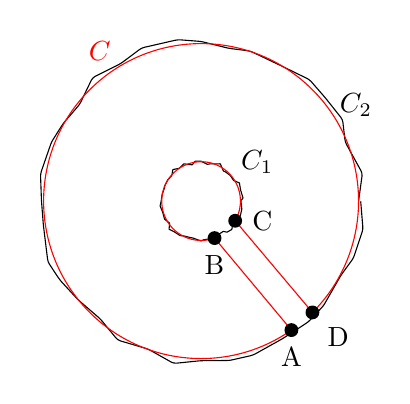
\begin{tikzpicture}
		\begin{scope}[decoration={random steps,segment length=10pt,amplitude=2pt}]
        \draw[decorate,rounded corners=1pt] (0,0) ellipse (2cm and 2cm) node [midway,label={[label distance=1.75cm]30:{$C_2$}}] {};
		\end{scope}
		\begin{scope}[decoration={random steps,segment length=2pt,amplitude=1pt}]
		\draw[decorate,rounded corners=0.1pt] (0,0) ellipse (0.5cm and 0.5cm) node [midway,label={[label distance=0.3cm]30:{$C_1$}}] {};
		\end{scope}
		\draw[color=red] (0, 0) ++(-45:2cm) arc (-45:305:2cm) node [midway,label=above:{$C$}] {} -- (290:0.5cm) arc (290:-30:0.5cm) -- (-45:2cm);
		\node[fill,circle,inner sep=0pt,minimum size=5pt,label=below:A] at (305:2cm) {};
		\node[fill,circle,inner sep=0pt,minimum size=5pt,label=below:B] at (290:0.5cm) {};
		\node[fill,circle,inner sep=0pt,minimum size=5pt,label=right:C] at (-30:0.5cm) {};
		\node[fill,circle,inner sep=0pt,minimum size=5pt,label=below right:D] at (-45:2cm) {};
	\end{tikzpicture}
	\caption{The contour $C$ in red, tracing out both $-C_1$ and $C_2$, connected via two curves $\gamma_{AB}$ and $\gamma_{CD}$.}
\end{figure}	

Let C be the contour $C_2 - AD + \gamma_{AB} - (C_1 - BC) + \gamma_{CD}$. By Cauchy's Theorem, $\oint_C f(z) \, dz = 0$. So:

\begin{align*}
0 &= \oint_{C_2} f - \int_A^D f + \int_A^B f - \oint_{C_1} + \int_B^C f + \int_C^D f \\
&= \oint_{C_2} f - \oint_{C_1} f + \left[ \int_A^B + \int_B^C + \int_C^D + \int_D^A \right] f \\
&\implies \oint_{C_1} f\,dz = \oint_{C_2} f\,dz
\end{align*}

\section{Cauchy's Integral Formula and Taylor Series}

For $f$ analytic on $D$, the integral of $f$ is invariant if the contour is deformed. 

\begin{example}{$f(z) = \frac{1}{z}$}

Let $C_1, C_2 = \left\{ z \rvert |z| = 1,2\right\}$. Parameterise $C_1$ by $z = e^{i\theta}$ and $C_2$ by $z = 2e^{i\theta}$. For $C_1$:

\[ dz = id\theta e^{i\theta} = izd\theta \]

So $\oint_{C_1} \frac{1}{z} \, dz = \int_0^{2\pi} \frac{iz}{z} \, d\theta = 2\pi i$

\end{example}

We find that $C_2$ gives the same answer, implying that the choice of contour does not change the value of the integral. 

\subsection{Cauchy's Integral Formula \book{24.10}}
\index{Cauchy's integral formula}

Let $f(z)$ be analytic on a simply connected domain $D$, with $C = \delta D$. Then for $z_0 \in D$:

\[ f(z_0) = \frac{1}{2\pi i} \oint_C \frac{f(z)}{z - z_0} \, dz \]

In other words, the value of a harmonic function inside a domain is determined by its value on the boundary. 

\subsubsection*{Proof}

$\frac{f(z)}{z - z_0}$ is not analytic in $D$ as it has a singularity at $z_0$. Let $C_\epsilon = \left\{ z \rvert \, |z - z_0 | = \epsilon \right\}$. By Cauchy corollary:

\begin{align*}
\oint_{C} \frac{f(z)}{z - z_0} \, dz &= \oint_{C_\epsilon} \frac{f(z)}{z - z_0} \, dz \\
&= \int^{2\pi}_0 \frac{f(z + \epsilon e^{i\theta})}{\cancel{\epsilon e^{i\theta}}} i \cancel{\epsilon e^{i\theta}} \, d\theta \\
&= i\int_0^{2\pi} d\theta \, f(z_0 + \epsilon e^{i\theta})
\end{align*}

But $f$ is continuous at $z_0$, hence

\[ \exists \delta \text{ s.t. } |f(z_0 + \epsilon e^{i\theta}) - f(z_0)| < \delta\]

So we can write $f(z_0 + \epsilon e^{i\theta}) = f(z_0) + \zeta$ where $|\zeta| < \delta$ and $|\zeta| \to 0$ as $\epsilon \to 0$. So:

\[ \oint_C \frac{f(z_0)}{z - z_0}\, dz = 2\pi i f(z_0) \]

Now consider $f'$:

\begin{align*}
f'(z_0) &= \lim_{\delta\to 0} \frac{f(z_0 + \delta) - f(z_0)}{\delta} \\
&= \lim_{\delta\to 0} \frac{1}{\delta} \frac{1}{2\pi i} \oint_C\left(\frac{f(z)}{z - (z_0 + \delta)} - \frac{f(z)}{z - z_0}\right)\, dz \\
&= \lim_{\delta\to 0} \frac{1}{\delta} \frac{1}{2\pi i} \oint_C f(z) \left(\frac{1}{z - z_0 - \delta} - \frac{1}{z - z_0}\right)\, dz \\
&= \lim_{\delta\to 0} \frac{1}{\cancel{\delta}} \frac{1}{2\pi i} \oint_C \frac{f(z)\cancel{\delta}}{(z-z_0)(z-z_0-\delta)}\, dz \\
&= \frac{1}{2\pi i}\oint_C \frac{f(z)}{(z-z_0)^2} \, dz
\end{align*}

In order to inductively find a general relation, assume that the following holds:

\begin{equation}\label{eq:integral_formula}
f^{(k)}(z_0) =  \frac{k!}{2\pi i } \oint_C \frac{f(z)}{(z - z_0)^{k+1}} \, dz 
\end{equation}

So, using the definition of the derivative:

\begin{align*}
f^{(k+1)}(z_0) &=  \lim_{\delta \to 0} \frac{f^{(k)}(z_0 + \delta) - f^{(k)}(z_0)}{\delta} \\
&= \lim_{\delta \to 0} \frac{1}{\delta} \frac{k!}{2\pi i} \oint_C \left[\frac{f^{(k)}(z_0)}{(z - z_0 - \delta)^{k+1}} - \frac{f(z_0)}{(z - z_0)^{k+1}}\right] \, dz \\
&= \lim_{\delta \to 0} \frac{1}{\delta} \frac{k!}{2\pi i} \oint_C f^{(k)}(z_0) \left[\frac{(z - z_0)^{k+1} - (z - z_0 - \delta)^{k + 1}}{(z - z_0 - \delta)^{k+1} (z-z_0)^{k+1}}\right] \, dz \\
&= \lim_{\delta \to 0} \frac{1}{\delta} \frac{k!}{2\pi i} \oint_C f^{(k)}(z_0) \left[\frac{z^{k+1} - (k+1)z^{k}z_0 + \dots - z^{k+1} + (k+1)z^{k}(z_0 + \delta) - ...}{(z - z_0 - \delta)^{k+1} (z-z_0)^{k+1}}\right] \, dz \\
&= \lim_{\delta \to 0} \frac{1}{\cancel{\delta}} \frac{(k+1)!}{2\pi i} \oint_C f^{(k)}(z_0) \left[\frac{\cancel{\delta}(z - z_0)^{k} + \mathcal{O}(\delta^2)}{(z - z_0 - \delta)^{k+1} (z-z_0)^{k+1}}\right] \, dz \\
&= \frac{(k+1)!}{2\pi i} \oint_C \frac{f(z_0)}{(z - z_0)^{k+2}} \, dz
\end{align*}

Hence the relation holds for $n = k + 1$ given that it holds for $n = k$. We have seen that it holds for $n = 0,1$ and so it is true for all $n \in \mathbb{N}$.

Thus, every analytic function is infinitely differentiable in its domain. 

\begin{example}{$f(z) = e^{2z}, C_2 = 2e^{i\theta}$}

We want to centre our contour on $z_0 = 1$:

\[ C_\epsilon = 1 + \epsilon e^{i\theta} \]

By Cauchy $\oint_{C_2} \frac{e^{2z}}{(z-1)^2} \, dz = \oint_{C_2} \frac{e^{2z}}{(z-1)^2} \, dz$. So we write $w = z - 1 = \epsilon e^{i\theta}$:

\begin{align*}
\oint_{C_2} \frac{e^{2z}}{(z-1)^2} \, dz &= \oint_{C_2} \frac{e^{2(w+1)}}{w^2} \, dz \\
&= \int_0^{2\pi} d\theta \, i\epsilon e^{i\theta} (e^{2w} \cdot e^2) w^{-2} \\
&= ie^{2} \int_{0}^{2\pi} d\theta \, \frac{e^{2w}}{w} \\
&= ie^2 \int_0^{2\pi} d\theta \, \left(\frac{1}{\epsilon e^{i\theta}} + 2 + \mathcal{O}(\epsilon)\right) \\
&= 4\pi e^2 \\
&= 2\pi i \cdot 2e^2 \\
&= 2\pi i f'(1)
\end{align*}
\end{example}

\subsection{Taylor Series \book{24.11}}
\index{Taylor series}

Let $f$ be analytic on a simply connected domain $D$. Then, for all $z \in D \, \exists r \text{ s.t. for } |z - z_0| < r$:

\[ f(z) = \sum_{n=0}^\infty \frac{f^{(n)}(z_0)}{n!} (z - z_0)^n \]

We will justify this using the following fact:

\begin{equation}\label{eq:epsilon}
\frac{1}{1-\epsilon} = \sum_{n=0}^\infty \epsilon^n \, \text{ for } |\epsilon| < 1
\end{equation} 

Consider:

\begin{align*}
\sum_{n=0}^\infty \frac{f^{(n)}(z_0)}{n!} (z - z_0)^n &= \sum_{n=0}^\infty \frac{1}{2\pi i} \oint_C \frac{f(\zeta) d\zeta}{(\zeta - z_0)^{n+1}} (z - z_0)^n \\
&= \frac{1}{2\pi i}\sum_{n=0}^\infty \oint_C \frac{f(\zeta)}{\zeta - z_0} \left(\frac{z - z_0}{\zeta - z_0}\right)^n d\zeta \\
\intertext{As  $z$ lies in the domain $D$ and $\zeta$ runs around its perimeter, we have \[ \left|\frac{z - z_0}{\zeta - z_0}\right| < 1\] So continuing from above and using Equation \ref{eq:epsilon}:} \\
&= \frac{1}{2\pi i} \oint_C \frac{f(\zeta)}{\zeta - z_0} \frac{d\zeta}{1 - \frac{z - z_0}{\zeta - z_0}} \\
&= \frac{1}{2\pi i} \oint_C \frac{f(\zeta)}{\zeta - z_0} d\zeta \footnotemark\\
&= f(z_0)\, \text{ (Cauchy formula)}
\end{align*}
\footnotetext{Here, we assume that $\left|\frac{z - z_0}{\zeta - z_0}\right| << 1$, however we have only specified that $\left|\frac{z - z_0}{\zeta - z_0}\right| < 1$. In the case that }

Note that whilst a finine polynomial in $z$ is entire, an infinite series may not converge. 

Suppose $P(z) = \sum_{n=0}^\infty a_n z^n$, then $P(n)$ converges if:

\[ \lim_{n\to\infty} \left|\frac{a_{n+1}}{a_n} z\right| < 1 \]

Hence 

\[ R = \frac{1}{\lim_{n\to\infty} \left|\frac{a_{n+1}}{a_n}\right|} \]

gives the radius of convergence of the series, meaning $P(z)$ converges as long as $z < R$.
\index{radius of convergence}

\begin{example}{$f(z) = \exp{z} = \sum_{n=1}^\infty \frac{z^n}{n!}$}
We have $a_n = \frac{1}{n!}$, so:

\begin{align*} 
\lim_{n\to\infty} \left|\frac{a_{n+1}}{a_n}\right| &= \lim_{n\to\infty} \left|\frac{n!}{(n+1)!}\right| \\
&= \lim_{n\to\infty} \frac{1}{n+1} \\
&= 0
\end{align*}

Hence $R \longrightarrow \infty$ so $\exp{z}$ is an entire function.
\end{example}

\section{Zeros and Poles}
\index{zeros}\index{poles}
\subsection{Liouville Theorem}
\index{Liouville theorem}

\begin{theorem}{Liouville Theorem}
Every bounded entire function is a constant.
\end{theorem}

\subsubsection*{Proof}

Consider Equation \ref{eq:integral_formula}. We see:

\begin{align*}
\left|f^{(n)}(z_0)\right| &= \frac{n!}{2\pi}\left|\oint_C \frac{f(z)}{(z-z_0)^{n+1}}\, dz\right| \\
&< \frac{n!}{2\pi}\oint_C \left| \frac{f(z)}{(z-z_0)^{n+1}}\, dz\right| \\
\intertext{Let $C = C_R = Re^{i\theta}$. Then, continuing from above:} \\
&< \frac{n!}{2\pi}\int_0^{2\pi} d\theta \, \frac{M}{R^n} \, \text{ where $|f(z)| < M, \, M\in \mathbb{R}^{+}$} \\
&= \frac{n!M}{R^n}
\end{align*}

Taking $R\to\infty$, we conclude $f^{(n)}(z_0) = 0 \, \forall n$ except $n=0$. So:

\begin{equation}
f(z) = \sum_{n=0}^\infty \frac{f^{(n)}(z_0)}{n!} (z-z_0)^n = f(z_0)
\end{equation}

\subsection{Zeros and Singularities \book{24.6}}
\index{zeros}

An analytic function $f(z)$ has a zero of multiplicity $n$ at $z_0$ if we can write 

\begin{equation}
f(z) = (z-z_0)^n g(z)
\end{equation}

where $g(z)$ is also analytic in the same domain. 

Suppose $f(z_0) = 0$ on a curve $\gamma \subset D, \, \gamma: [a,b] \to D$, and $z_0 = \gamma(t_0)$. Consider:
\[ \frac{df}{dz} - \lim_{\delta\to 0} \frac{f(z+\delta) - f(z)}{\delta}\]

Let $z_0 + \delta = \gamma(t_0 + \epsilon)$, where $\epsilon \to 0$ as $\delta \to 0$. Then
\[ f(z_0 + \delta) \to f(z_0) = 0 \implies \left.\frac{df}{dz}\right|_{z_0} = 0 \]

Our choice of $z_0$ is not unique, so this is true for all points on $\gamma$. By iteration, $f^{(n)}(z) = 0 \, \forall z \in \gamma$, i.e. $f \equiv 0$. Hence the zeros of an analytic function are isolated, as the existence of two zeros at $z_0$ and $z_0 + \delta$ for arbitrarily small $\delta$ implies $f$ is trival.

\index{poles}
Let $f$ be analytic in a domain $D/\{z_0\}$. Then $f$ has a pole of order $m$ at $z_0$ if we can write

\begin{equation}
f(z) = \frac{g(z)}{(z - z_0)^m}
\end{equation}

where $g$ is analytic in $D$ and $g(z_0) \neq 0$. 

Consider a function:

\[ f(z) = f(z_0) + (z-z_0)f'(z_0) + \frac{1}{2}(z-z_0)^2f''(z_0) + \dots \]

Dividing by $(z-z_0)^n$ and taking the contour integral:

\begin{align*} \oint_C \frac{f(z)}{(z-z_0)^n}\, dz &= \oint_C \underbrace{\frac{f(z_0)}{(z-z_0)^n} + \frac{f'(z_0)}{(z-z_0)^{n-1}} + \dots}_\text{vanishes\footnotemark} + \frac{1}{(n-1)!}\frac{f^{(n-1)}(z_0)}{z - z_0} \\ 
&\underbrace{ + \frac{1}{n!}f^{(n)}(z_0) + \frac{(z - z_0)}{(n+1)!}f^{(n+1)}(z_0) + \dots}_\text{vanishes\footnotemark} \, dz \\
&= \frac{1}{(n-1)!} \oint_C \frac{f^{(n-1)}(z_0)} \, dz \\
&= \frac{2\pi i}{(n-1)!} f^{(n-1)}(z) \end{align*}

\footnotetext[2]{From Equation \ref{eq:integral_formula}, \[\frac{1}{n!}f^{(n)}(z_0) = \frac{1}{2\pi i}\oint_C \frac{f(z)}{(z - z_0)^{n+1}}\] so \[\frac{1}{i!}\frac{f^{(i)}(z_0)}{(z-z_0)^{n-i}} =  \frac{1}{(z - z_0)^{n-i}} \oint_C \frac{f(z_0)}{(z - z_0)^{i+1}}\, dz = 0\] as \[ \oint_C \frac{1}{(z - z_0)^{i+1}}\, dz = 2\pi i \left.\frac{\partial^i}{\partial z^i} 1\right|_{z_0} = 0\] for $i \neq 0$, which is the only term that remains.}
\footnotetext[3]{This forms an analytic function.}

which agrees with Cauchy's integral formula. Hence, only the $\frac{1}{z - z_0}$ term contributes to the contour integral. 

\section{Meromorphic Functions and Laurent Series}
\index{meromorphic functions}

A function is \emph{meromorphic} in a domain $D$ if it is holomorphic (analytic) except for poles. 

Consider the definition of a pole:

\begin{align*}
f(z) &= \frac{g(z)}{(z - z_0)^n} \text{ for holomorphic } g \\
&= \frac{\sum^\infty_{n=0}g_n (z-z_0)^n}{(z-z_0)^m} \\
&= \sum_{n=-m}^\infty g_{n+m} (z - z_0)^n
\end{align*}

This resembles a Taylor series, but with negative powers of $(z-z_0)$.

\section{Laurent series \book{24.11}}
\index{Laurent series}
\index{Laurent's theorem}

\begin{theorem}{Laurent's theorem}
Let $f(z)$ be analytic in the annulus
\[ {|z-z_0| \in (r_1 , r_2)} \]

with $f$ undefined at $z_0$. Then

\begin{align*}
f(z) &= \sum_{n=-\infty}^\infty a_n (z-z_0)^n \\
&= \underbrace{\sum_{n=0}^\infty a_n (z-z_0)^n}_\text{regular `Taylor' part} + \underbrace{\sum_{n=-\infty}^{-1} a_{n}(z-z_0)^n}_\text{principal part}
\end{align*}

where $a_n = \frac{1}{2\pi i} \oint_C \frac{f(z)}{(z-z_0)^{n+1}}\, dz$ and $C$ is any simple, closed, non-contractible contour within the annulus.

\end{theorem}

\subsubsection*{Proof}

Without loss of generality, let $z_0 = 0$. Then

\begin{align*}
f(z) &= \frac{1}{2\pi i} \oint_{C'} \frac{f(\zeta)}{\zeta - z}\, d\zeta \\
&\text{where $C'$ is a simple curve around some $z$} \\
&= \frac{1}{2\pi i} \oint_{C_2} \frac{f(\zeta)}{\zeta - z}\, d\zeta - \frac{1}{2\pi i} \oint_{C_1} \frac{f(\zeta)}{\zeta - z}\, d\zeta \\
&=\text{by similar argument to Cauchy's theorem}
\end{align*}

Now consider the two terms separately:

\begin{align*}
f_1 (z) &= \frac{1}{2\pi i} \oint_{C_2} \frac{f(\zeta)}{\zeta - z}\, d\zeta \\
&= \frac{1}{2\pi i} \oint_{C_2} \frac{f(\zeta)}{\zeta} \sum_{n=0}^\infty \left(\frac{z}{\zeta}\right)^n d\zeta \text{ using \ref{eq:epsilon}}\\
&= \frac{1}{2\pi i} \oint_{C_2} \frac{f(\zeta)}{\zeta} \left[ \sum_{n=0}^N \left(\frac{z}{\zeta}\right)^n + \left(\frac{z}{\zeta}\right)^N \sum_{n=0}^\infty \left(\frac{z}{\zeta}\right) \right] \, d\zeta \\
&= \frac{1}{2\pi i }\sum_{n=0}^N \oint_{C_2} \frac{f(\zeta)}{\zeta} \left(\frac{z}{\zeta}\right)^n d\zeta + \frac{1}{2\pi i}\oint_{C_2} \frac{f(\zeta)}{\zeta} \left(\frac{z}{\zeta}\right)^N \sum_{n=0}^\infty \left(\frac{z}{\zeta}\right)^n d\zeta \\
&= \sum_{n=0}^N a_n z^n + \frac{1}{2\pi i} \oint_{C_2} \frac{f(\zeta)}{\zeta - z} \left(\frac{z}{\zeta}\right)^N \, d\zeta
\end{align*}

However

\begin{align*} 
\left|\frac{1}{2\pi i} \oint_{C_2} \frac{f(\zeta)}{\zeta - z} \left(\frac{z}{\zeta}\right)^N \, d\zeta \right| &< \frac{1}{2\pi} \oint_{C_2} \underbrace{\left|\frac{f(\zeta)}{\zeta - z}\right|}_{M} \underbrace{\left|\frac{z}{\zeta}\right|^N}_{\epsilon^N} \left|d\zeta\right| \\
&\to 0
\end{align*}

as $N\to \infty$, hence in the limit $N\to\infty$, $f_1(z) = \sum_{n=0}^\infty a_n z^n$.

Similarly:

\begin{align*}
f_2 (z) &= -\frac{1}{2\pi i} \oint_{C_1} \frac{f(\zeta)}{\zeta - z} \, d\zeta \\
&= \frac{1}{2\pi i} \oint_{C_1} \frac{f(\zeta)}{z} \sum_{n=0}^\infty \left(\frac{\zeta}{z}\right)^n \, d\zeta \\
&= \frac{1}{2\pi i} \sum_{n=0}^\infty \oint_{C_1} \frac{f(\zeta)}{z} \left(\frac{\zeta}{z}\right)^n \, d\zeta \\
\intertext{By a similar argument to above:}
&= \frac{1}{2\pi i} \sum_{n=-\infty}^{-1} \oint_{C_1} \frac{f(\zeta)}{z} \left(\frac{\zeta}{z}\right)^{-n-1} \, d\zeta \\
&= \frac{1}{2\pi i} \sum_{n=-\infty}^{-1} \oint_{C_1} z^n \left(\frac{f(\zeta)}{\zeta^{n+1}}\right)^{-n-1} \, d\zeta \\
&= \sum_{n=-\infty}^{-1} a_n z^n
\end{align*}

Putting both together:

\[ f(z) = f_1 (z) + f_2 (z) = \sum_{-\infty}^{\infty} a_n z^n \]

Note $f_1$ is holomorphic for $|z| < r_2$ and $f_2$ is holomorphic for $|z|>r_1$.

Clearly, if $f$ has a pole at $z_0$, the Laurent series will terminate at some $n = -m$, where $m$ is the order of the pole. However, if the series does not terminate, then we say $f(z)$ has an essential singularity at $z_0$.

\begin{example}{$f(z) = \exp{\frac{1}{z}}$}

\begin{align*}
f(z) &= \exp{\frac{1}{z}} \\
&= \sum_{n=0}^\infty \frac{\left(\frac{1}{z}\right)^n}{n!} \\
&= \sum_{n=-\infty}^0 \frac{z^n}{|n|!}
\end{align*}

The singularity is `nasty' in the sense that $f$ takes all possible complex values in a neighbourhood of $z_0$, except possibly for 1. As $z\to 0$:

\begin{align*}
f(x) &= e^{\frac{1}{x}} \to \begin{cases} \infty & \mbox{if } x>0 \\
0 & \mbox{if } x<0 \end{cases} \\
f(iy) &= e^{-\frac{i}{y}} = \cos{\frac{1}{y}} - i\sin{\frac{1}{y}}
\end{align*}
\end{example}

\subsection{Integrating a meromorphic function \book{24.12}}\label{sec:evaluating_poles}
\index{integration}\index{meromorphic functions}

The poles of a meromorphic function are isolated (of a similar vein to isolated zeros). We can use Laurent series to evaluate contour integrals:

\[ \oint_C f(z)\, dz = \oint_C dz \left(\sum_{n=0}^\infty a_n (z-z_0)^n + \sum_{n=\infty}^{-1} a_n (z-z_0)^n \right) \]

For the principal part:

\[ \oint_C (z-z_0)^n \, dz = \begin{cases} 0 & \mbox{if } n\neq -1 \\ 2\pi i & \mbox{if } n = 1 \end{cases}\]

So 

\begin{equation}
\oint_C f(z)\, dz = 2\pi i a_{-}
\end{equation} 

We refer to $a_{-}$ as the residue of $f(z)$ at $z_0$. The optimal method to calculate the residue depends on the situation:
\index{residues}

\begin{enumerate}[label=\alph*)]
\item{Simple poles \[ f(z) = \frac{g(z)}{z - z_0} \text{, $g$ holomorphic at $z_0$, $g(z_0) \neq 0$}\] \[ Res[f, z_0] = g(z_0) = \lim_{z\to z_0} (z - z_0)f(z) \]}
\item{Pole of order $n$ \[ f(z) = \frac{g(z)}{(z - z_0)^n} \text{, $g$ holomorphic at $z_0$, $g(z_0) \neq 0$}\] We need the $(n-1)$th coefficient of the Taylor series of $g$: \[ Res[f, z_0] = \frac{g^{(n-1)} (z_0)}{(n-1)!} = \frac{1}{(n-1)!}\lim_{z\to z_0} \frac{d^{n-1}}{dz^{n-1}}\left( (z - z_0)^n f(z)\right) \]}
\item{$f(z) = \frac{g(z)}{h(z)}$, $g,h$ holomorphic, $h$ has simple zero at $z_0$ \[ Res[f, z_0] = \frac{g(z_0)}{h'(z_0)}\]}
\end{enumerate}
\index{poles}

If $z_0$ is not a simple pole, then it is safest to series expand and use $\frac{1}{1-\epsilon}$ formula as required.

\begin{example}{$f(z) = \frac{1}{z(z-1)}$}

Using partial fractions, we can rewrite $f(x)$ to identify its $\frac{1}{z-a}$ components:

\[ f(z) = \frac{1}{z(z-1)} = -\frac{1}{z} + \frac{1}{z-1} \]

We see that $f(z)$ has simple poles at $z = 0$ and $z = 1$. Now we will consider the contour integral:

\begin{align*}
	\oint_C f(z)\, dz &= \oint_C \frac{dz}{z(z-1)} \\
	&= \oint_C dz\,\left[-\frac{1}{z}+\frac{1}{z-1}\right] \\
	&= -\oint_C \frac{dz}{z} + \oint_C \frac{dz}{z-1}
\end{align*}

For the contour $C_2 = 2e^{i\theta}$, both poles lie inside and so both of the contour integrals on the right contribute $2\pi i$, giving a result of zero. For $C_\frac{1}{2} = \frac{1}{2}e^{i\theta}$, only the $\frac{1}{z}$ component contributes so the result is $-2\pi i$.

\end{example}

\begin{example}{$f(z) = \frac{e^{2z}}{z^2 - 4}$}

We can write:

\[ f(z) = \frac{e^{2z}}{z^2 - 4} = \frac{e^{2z}}{(z+2)(z-2)} \]

So we see that $f(z)$ has simple poles at $z_0=\pm 2$. We then evaluate the residues:

\begin{enumerate}[label={$z_0=\arabic*$:}]
	\setcounter{enumi}{1}
	\item{
		\begin{align*}
			Res[f,2] &= \lim_{z\to 2} (z-2) f(z) \\
			&= \lim_{z\to 2} \frac{e^{2z}}{z+2} \\
			&= \frac{e^4}{4}
		\end{align*}
	}
	\setcounter{enumi}{-3}
	\item{
		\begin{align*}
			Res[f,-2] &= \lim_{z\to -2} (z+2) f(z) \\
			&= \lim_{z\to 2} \frac{e^{2z}}{z-2} \\
			&= \frac{e^{-4}}{-4}
		\end{align*}
	}
\end{enumerate}

Consider the following contours:

\begin{align*}
	C &= 1 + 2e^{i\theta} \\
	C' &= 3e^{i\theta} 
\end{align*}

Both poles lie inside $C'$, but only $z=2$ lies in $C$, hence:

\begin{align*}
	\oint_C f(z)\, dz &= 2\pi i \left[\frac{e^4}{4}\right] \\
	&= \frac{\pi i e^4}{2} \\
	\oint_{C'} f(z)\, dz &= 2\pi i \left[\frac{e^4}{4} - \frac{e^{-4}}{4}\right] \\
	&= \pi i \sinh{4}
\end{align*}
\end{example}

\begin{example}{$f(z) = \frac{1}{z\sin z}$}

This has a pole of order 2 at $z_0 = 0$. Using the Talor expansion \[ \sin z = z - \frac{z^3}{3!} + \dots \] we have 

\begin{align*} 
f(z) &= \frac{1}{z\left(z - \frac{z^3}{3!} + \dots \right)} \\
&= \frac{1}{z^2 \left(1 - \frac{z^2}{3!} + \dots \right)} \\
\intertext{Using Equation \ref{eq:epsilon}} \\
&= \frac{1}{z^2}\left(1 + \frac{z^2}{3!} + \dots \right) \\
&= \frac{1}{z^2} + \frac{1}{3!} + \dots
\end{align*}

We see there is no $\frac{1}{z}$ component, and so $Res[f,0] = 0$.

\end{example}

\begin{theorem}{Residue Theorem}

Let $f$ be a meromorphic function with poles at ${z_i}$. Then

\[ \oint_C f(z)\, dz = 2\pi i \sum_i Res[f,z_i] \]

\end{theorem}

\subsubsection*{Proof (Sketch)}

\begin{figure}
\centering
	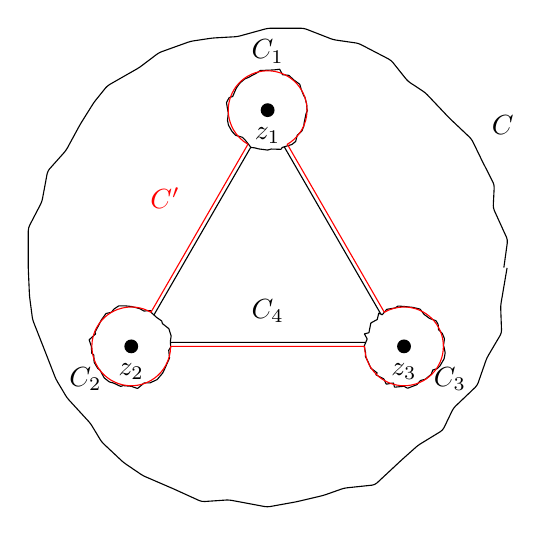
\begin{tikzpicture}
		% Set up coordinates to draw
		\newcommand{\aaa}{(0,0) ++(90:2cm)}
		\newcommand{\bbb}{(0,0) ++(210:2cm)}
		\newcommand{\ccc}{(0,0) ++(330:2cm)}

		\draw (0,0) ++(90:1.9cm) -- +(-60:3.2909cm) -- node [midway,label=above:{$C_4$}] {} +(240:3.2909cm) -- cycle;

		\begin{scope}[decoration={random steps,segment length=10pt,amplitude=2pt}]
        \draw[decorate,rounded corners=1pt] (0,0) ellipse (3cm and 3cm) node [midway,label={[label distance=3cm]30:{$C$}}] {};
		\end{scope}
		\begin{scope}[decoration={random steps,segment length=2pt,amplitude=1pt}]
		\draw[decorate,rounded corners=0.1pt,fill=white] \aaa ellipse (0.5cm and 0.5cm) node [midway,label={[label distance=2.35cm]90:{$C_1$}}] {};
		\draw[decorate,rounded corners=0.1pt,fill=white] \bbb ellipse (0.5cm and 0.5cm) node [midway,label={[label distance=2.15cm]210:{$C_2$}}] {};
		\draw[decorate,rounded corners=0.1pt,fill=white] \ccc ellipse (0.5cm and 0.5cm) node [midway,label={[label distance=2.15cm]330:{$C_3$}}] {};
		\end{scope}
		\node[fill,circle,inner sep=0pt,minimum size=5pt,label=below:{$z_1$}](z1) at ++(90:2cm) {};
		\node[fill,circle,inner sep=0pt,minimum size=5pt,label=below:{$z_2$}](z2) at ++(210:2cm) {};
		\node[fill,circle,inner sep=0pt,minimum size=5pt,label=below:{$z_3$}](z3) at ++(330:2cm) {};
		\draw[red] (z1) ++(240:0.5cm) -- ++(240:2.464101615cm) node [midway,label=above left:{$C'$}] {} arc (60:360:0.5cm) -- ++(0:2.464101615cm) arc (-180:120:0.5cm) -- ++(120:2.464101615cm) arc (-60:240:0.5cm);
	\end{tikzpicture}
\caption{The contour $C$ in red, tracing out $C_1$, $C_2$ and $C_3$ which are centred on poles $z_1$, $z_2$ and $z_3$ respectively, and $C_4$ which comprises the three lines that connect them.}\label{fig:residue_theorem}
\end{figure}

\begin{align*} 
\oint_C f(z)\, dz &= \oint_{C'} f(z)\, dz \\
&= \left[ \oint_{C_1} + \oint_{C_2} + \oint_{C_3} + \oint_{C_4} \right] f\, dz
\end{align*}

\section{Contour Integration}
\index{contours}
\index{integration}
\index{contour integration}

\subsection{Examples}
\begin{enumerate}[label=\alph*)]
\item{$f(z) = \frac{\cos{\pi z}}{z^2 (1-z)}$, which has a simple pole at $z=1$ and a double pole at $z=0$. We now evaluate residues:

\begin{align*}
z_0 = 1: \hspace{1cm}  Res[f,1] &= \lim_{z\to 1} (z-1) f(z) \\
&= \lim_{z\to 1} -\frac{\cos{\pi z}}{z^2} = 1 \\
z_0 = 0: \hspace{1.7cm}  f(z) &= \frac{g(z)}{z^2} = \frac{\cos{\pi z}}{1 - z} \\
\intertext{ Taylor expanding $g(z)$ around $z_0$: \begin{align*} \frac{\cos{\pi z}}{1-z} &= (1 - \frac{1}{2}(\pi z)^2 + \dots)(1 + z + z^2) \\ &= 1 + z + z^2 - \frac{1}{2}\pi^2 z^2 + \dots \end{align*}}
f(z) &= \frac{1}{z^2} + \underbrace{\frac{1}{z}}_{Res[f,0] = 1} + 1 - \frac{1}{2}\pi^2 z^2 + \dots
\end{align*}

So

\begin{align*}
\oint_{C_\frac{1}{2}} f(z)\, dz &= 2\pi i Res[f,0] = 2\pi i \\
\oint_{C_2} f(z)\, dz &= 2\pi i \left\{Res[f,0] + Res[f,1] \right\} = 4\pi i
\end{align*}}
\item{$f(z) = \frac{e^z}{z^2 + z + 1}$, which has simple poles at roots of $z^2 + z + 1 = 0$:
\[ z_\pm = -\frac{1}{2} \pm \frac{1}{2}\sqrt{1 - 4} = -\frac{1}{2} \pm i\frac{\sqrt{3}}{2} = e^{\pm\frac{2\pi i}{3}} \]

Hence $f$ has two simple poles on the unit circle. Evaluating residues:

\begin{align*}
z_0 = e^\frac{2\pi i }{3}: \hspace{1cm} Res[f,e^\frac{2\pi i}{3}] &= \lim_{z\to e^\frac{2\pi i}{3}} (z - e^\frac{2\pi i}{3})f(z) \\ 
&= \lim_{z\to e^\frac{2\pi i}{3}} \frac{e^z}{z - e^\frac{-2\pi i}{3}} \\ 
&= \frac{e^{-\frac{1}{2}} e^{i\frac{\sqrt{3}}{2}}}{e^\frac{2\pi i}{3} - e^\frac{-2\pi i}{3}} \\
&= \frac{e^{-\frac{1}{2}} (\cos{\frac{\sqrt{3}}{2}} + i\sin{\frac{\sqrt{3}}{2}}) }{i\sqrt{3}} \\
z_0 = e^\frac{-2\pi i}{3}: \hspace{1cm} Res[f,e^\frac{-2\pi i}{3}] &= \lim_{z\to e^\frac{-2\pi i}{3}} (z - e^\frac{-2\pi i}{3})f(z) \\ 
&= \lim_{z\to e^\frac{-2\pi i}{3}} \frac{e^z}{z - e^\frac{2\pi i}{3}} \\ 
&= \frac{e^{-\frac{1}{2}} e^{-i\frac{\sqrt{3}}{2}}}{e^\frac{-2\pi i}{3} - e^\frac{2\pi i}{3}} \\
&= \frac{e^{-\frac{1}{2}} (\cos{\frac{\sqrt{3}}{2}} - i\sin{\frac{\sqrt{3}}{2}}) }{-i\sqrt{3}}
\end{align*}

So for $R>1$: \begin{align*} 
\oint_{C_R} f(z)\, dz &= 2\pi i \left\{Res[f,e^\frac{2\pi i }{3}] + Res[f, e^{-\frac{2\pi i}{3}}]\right\} \\
&= 2\pi i \left\{ \frac{e^{-\frac{1}{2}} (\cos{\frac{\sqrt{3}}{2}} + i\sin{\frac{\sqrt{3}}{2}}) }{i\sqrt{3}} + \frac{e^{-\frac{1}{2}} (\cos{\frac{\sqrt{3}}{2}} - i\sin{\frac{\sqrt{3}}{2}}) }{-i\sqrt{3}} \right\} \\
&= \frac{4\pi i}{\sqrt{3}} \sin{\frac{\sqrt{3}}{2}}
\end{align*}
}
\end{enumerate}

\index{poles}\index{zeros}\index{poles and zeros theorem}
\begin{theorem}{`Poles and Zeros' Theorem}
Let $f$ be meromorphic inside a contour C, then

\begin{equation}\label{thm:poles_and_zeros}
\frac{1}{2\pi i} \oint_C dz \, \frac{f'(z)}{f(z)} = n_\text{zeros} - n_\text{poles} \text{, including multiplicity}
\end{equation}

\end{theorem}

\subsubsection*{Proof}

First note that if $f(z)$ has a pole of order $n$ at $z_0$ then $f'(z)$ will have a pole of $n+1$ as $z_0$, meaning $\frac{f'(z_0)}{f(z_0)}$ will look like a simple pole. 

Now let $f(z)$ have a zero of multiplicity $n$ at $z_0$, meaning $f(z) = (z-z_0)^n g(z)$. So:
\begin{align*} 
\frac{f'(z)}{f(z)} &= \frac{n(z-z_0)^{n-1} g + (z-z_0)^n g'}{(z-z_0)^n g} \\
&= \frac{n}{z-z_0} + \underbrace{\frac{g'(z)}{g(z)}}_\text{Disappears according to Cauchy's theorem}
\end{align*}
So $\frac{1}{2\pi i}\oint_C \frac{f'(z)}{f(z)}\, dz = n$.

Similarly for a pole of order $m$, $f(z) = \frac{g(z)}{(z-z_0)^m}$ and $\frac{f'(z)}{f(z)} = -\frac{m}{z-z_0} + \frac{g'(z)}{g(z)}$. Therefore $\frac{1}{2\pi i}\oint_C \frac{f'(z)}{f(z)}\, dz = -m$, and so the result follows. 

\subsection{Trigonometric Integrals \book{24.13.1}}
\index{integration}\index{trigonometric functions}\index{trigonometric integrals}\index{real integrals}

Consider an integral of the form 
\[ I = \int_{0}^{2\pi} d\theta R(\cos{m\theta}, \sin{n\theta}) \]
where $R$ is a rational function (ratio of polynomials). We can reinterpret this as a contour integral around the unit circle and use the methods we have seen so far to solve it. 

By expressing $z = e^{i\theta}$, we have $\frac{dz}{iz} = d\theta$ so $\int_{0}^{2\pi}d\theta$ becomes $\oint_{C_1} \frac{dz}{iz}$. We also perform the following substitutions:

\begin{align*}
\cos{m\theta} &= \frac{1}{2}\left[e^{im\theta} + e^{-im\theta}\right] \\
&= \frac{1}{2}\left[z^m + z^{-m}\right] \\
\sin{n\theta} &= \frac{1}{2i}\left[e^{in\theta} - e^{-in\theta}\right] \\
&= \frac{1}{2i}\left[z^n + z^{-n}\right] 
\end{align*}

Thus our integral becomes:

\[I = \oint_{C_1} -i \frac{dz}{z} R(\frac{z^m + z^{-m}}{2}, \frac{z^n - z^{-n}}{2})\]

Unless $R$ is a very simple function, the contour integral is going to be easier to deal with than the real integral. 

\begin{example}{}
\begin{enumerate}
\item{
	\begin{align*}
		I = \int_0^{2\pi} \frac{d\theta}{2-\cos{\theta}} &\rightarrow \oint_{C_1} -\frac{idz}{z} \frac{1}{2 - \frac{z + z^{-1}}{2}} \\
		&= \oint_{C_1} \frac{2idz}{z^2 - 4z + 1}
	\end{align*}

	This quadratic has roots at $z_\pm = 2\pm\sqrt{3}$. We discount $z_+ = 2+\sqrt{3}$ as it is clearly outside of the unit circle, and so by Theorem \ref{thm:poles_and_zeros} will not contribute to the contour integral. 

	We now evaluate the remaining residue:

	\begin{align*}
		Res[f, 2-\sqrt{3}] &= \lim_{z\to 2-\sqrt{3}} \frac{2i}{z-2-\sqrt{3}} \\
		&= -\frac{i}{\sqrt{3}}
	\end{align*}
	
	So $I = 2\pi i \cdot -\frac{i}{\sqrt{3}} = \frac{2\pi}{\sqrt{3}}$.	
}
\item{
	\begin{align*}
		I &= \int_0^{2\pi} \frac{d\theta \sin{\theta}}{(3+\cos{\theta})(2+\sin{\theta})} \\
		&= \oint_{C_1} -\frac{idz}{z} \frac{\frac{z - z^{-1}}{2i}}{(3 + \frac{z + z^{-1}}{2})(2 + \frac{z - z^{-1}}{2i})} \\
		&= \oint_{C_1} -2idz \frac{z^2 - 1}{\underbrace{(z^2 + 6z + 1)}_{z_\pm = -3\pm 2\sqrt{2}} \underbrace{(z^2 + 4iz - 1)}_{z_\pm = -2i \pm i\sqrt{3}}}
	\end{align*}

	We discount poles that lie outside $C_1$, so we are left with poles at $z_1 = -3 + 2\sqrt{2}$ and $z_2 = -2i + i\sqrt{3}$. First, evaluate the following:

	 \[
	 	z_1^2 = 17 - 12\sqrt{2}
 	\] 
 	\begin{align*}
 		z_1^2 - 1 &= 16 - 12\sqrt{2} \\
 		&= 4\sqrt{2}(2\sqrt{2} - 3) \\
 		&= 4\sqrt{2}z_1
 	\end{align*}

 	So

 	\begin{align*}
 		Res[f, 2\sqrt{2} - 3] &= \lim_{z\to 2\sqrt{2} - 3} (z + 3 - 2\sqrt{2})f(z) \\
 		&= \left.\frac{-2i(z^2 - 1)}{(z^2 + 4iz - 1)(z + 3 + 2\sqrt{2})}\right|_{z_1} \\
 		&= \frac{2i \cancel{4\sqrt{2}}\cancel{z_1}}{(4\sqrt{2}\cancel{z_1} + 4i\cancel{z_1})\cancel{4\sqrt{2}}} \\
 		&= \frac{-2i}{4(\sqrt{2} + i)} \\
 		&= \frac{-2i \cdot (\sqrt{2} - i)}{12} \\
 		&= \frac{-i(\sqrt{2} - i)}{6}
	\end{align*}

	Similarly for $z_2 = -2i + i\sqrt{3}$, we evaluate:

	\[
	 	z_2^2 = -(7-4\sqrt{3})
 	\] 
 	\begin{align*}
 		z_2^2 + 1 &= -6 + 4\sqrt{3} \\
 		&= 2\sqrt{3}(\sqrt{3} - 2) \\
 		&= -2\sqrt{3}\frac{z_2}{i} \\
 		&= 2\sqrt{3}iz_2
 	\end{align*}
 	\begin{align*}
 		z_2^2 - 1 &= -8 + 4\sqrt{3} \\
 		&= 4(-2 + \sqrt{3}) \\
 		&= -4iz_2
 	\end{align*}

 	So 

 	\begin{align*}
 	Res[f,-2i + i\sqrt{3}] &= \lim_{z\to -2i + i\sqrt{3}} (z + 2i - i\sqrt{3})f(z) \\
 	&= \left.\frac{-2i(z^2 - 1)}{(z^2 + 6z + 1)(z + 2i + i\sqrt{3})}\right|_{z_2} \\
 	&= \frac{-2i \cdot -4iz_2}{z_2 (2i\sqrt{3} + 6)\cdot 2i\sqrt{3}} \\
 	&= \frac{2i}{3(\sqrt{3} + i)} \\
 	&= \frac{i(\sqrt{3} - i)}{6}
 	\end{align*}

 	Hence 

 	\begin{align*}
 	I &= 2\pi i \cdot \left[\frac{i(\sqrt{3} - i)}{6} - \frac{i(\sqrt{2}-i)}{6}\right] \\
 	&= \frac{2\pi i}{6}\left[i\sqrt{3} - i\sqrt{2}\right] \\
 	&= \frac{\pi}{3}(\sqrt{2} - \sqrt{3})
 	\end{align*}
}

\end{enumerate}
\end{example}

\section{Integrals over $\mathbb{R}$}
\index{real integrals}

\subsection{$\mathbb{R}$ Integrals \book{24.13.2}}

Consider $I = \int_{-\infty}^\infty \frac{dx}{x^2 + 1}$. We will solve using two methods:

\begin{enumerate}[label=\alph*)]
	\item{
		$\mathbb{R}$ method \newline

		Let $x = \tan{u} \implies dx = \sec^2{u}\, du = (1+\tan^2{u})du$. So $I = \int_{-\frac{\pi}{2}}^{\frac{\pi}{2}} du = \pi $.
	}

	\item{
		$\mathbb{C}$ method \newline

		Let $f(z) = \frac{1}{z^2 + 1}$.

		Currently our `contour' is the real line, meaning we need to close it in order to perform contour integration. Consider the contour $C_R = [-R, R]\cup \left\{Re^{i\theta}\right\}, \theta \in (0,\pi)$ (traversed anticlockwise), shown in Figure \ref{fig:semicircle_contour}.

		We see that $f(x) = \frac{1}{z^2 + i} = \frac{1}{(z+i)(z-i)}$, i.e. $f(x)$ has poles at $z_0 = \pm i$. Since $-i$ lies outside our contour, we only need to find one residue:

		\begin{align*}
			Res[f,i] &= \lim_{z\to i} (z - i)f(z) \\
			&= \lim_{z\to i} \frac{1}{z + i} \\
			&= \frac{1}{2i}
		\end{align*}

		So $I = 2\pi i Res[f,i] = \pi$. However, we also need to consider the contribution of the semi-circular portion of the contour. We see

		\begin{align*}
			\left|\int_{Re^{i\theta}} dz\, f(z)\right| &< \int_0^{\pi} \frac{R}{|R^2 e^{2i\theta} + 1|} \\
			&= \frac{1}{R}\int_0^{\pi} \frac{1}{|e^{2i\theta} + \frac{1}{R^2}|} \\
			&< \frac{\pi}{R} \to 0 \text{ as } R \to \infty 
		\end{align*}

		Therefore in the limit $R\to\infty$, $I = \oint_{C_R} f(z)\, dz = \pi$. 
	}
\end{enumerate}

\begin{figure}
	\centering
	\begin{tikzpicture}
    \begin{scope}[thick,font=\scriptsize,decoration={markings,mark=at position 0.6 with {\arrow{>}}}]
    % Axes:
    % Are simply drawn using line with the `->` option to make them arrows:
    % The main labels of the axes can be places using `node`s:
    \draw [->,postaction={decorate}] (-2,0) -- (2,0) node [above]  {$\Re\{z\}$};
    \draw [->] (0,-2) -- (0,2) node [left] {$\Im\{z\}$};

    % Axes labels:
    \draw (1,-3pt) -- (1,3pt)   node [below right] {$R$};
    \draw (-1,-3pt) -- (-1,3pt) node [below left] {$-R$};

    % Draw curved portion of semicircle
    \draw[postaction={decorate}] (1,0) arc (0:180:1cm);
    
    \end{scope}
	\end{tikzpicture}
	\caption{The semicircular contour $C_R = [-R, R]\cup \left\{Re^{i\theta}\right\}, \theta \in (0,\pi)$.}
	\label{fig:semicircle_contour}
\end{figure}

\begin{example}{$I = \int_{-\infty}^\infty \frac{x+2}{(2x^2 + 3)^2}\, dx$}
	Let $f(z) = \frac{z + 2}{(2z^2 + 3)^2}$. Notice $|f(z)| < \frac{1}{R^3}$ for large $|z| = R$. Thus, the integral of $f(z)$ around any portion of the circle $|z| = R$ goes to zero as $R\to\infty$. 

	Hence $I = \oint_{C_R} f(z)\, dz$. $f(z)$ has double poles at $z = \pm i\sqrt{\frac{3}{2}}$. Neglecting $z = -i\sqrt{\frac{3}{2}}$ as it lies outside the contour, we have:

	\begin{align*}
		Res[f,i\sqrt{\frac{3}{2}}] &= \lim_{z\to i\sqrt{\frac{3}{2}}} \frac{d}{dz}\left[(z - i\sqrt{\frac{3}{2}})f(z)\right] \\
		&= \lim_{z\to i\sqrt{\frac{3}{2}}} \frac{d}{dz}\left[\frac{z+2}{4(z+i\sqrt{\frac{3}{2}})^2}\right] \\
		&= \lim_{z\to i\sqrt{\frac{3}{2}}} \left[\frac{1}{4(z + i\sqrt\frac{3}{2})^2} - \frac{z+2}{2(z + i\sqrt{\frac{3}{2}})^3}\right] \\
		&= \frac{1}{4(2i\sqrt{\frac{3}{2}})^2} - \frac{2 + i\sqrt{\frac{3}{2}}}{2(2i\sqrt{\frac{3}{2}})^3} \\
		&= -\cancel{\frac{1}{24}} - \frac{i}{6\sqrt{6}} + \cancel{\frac{1}{24}}
	\end{align*}

	So $\int_{C_R} f(z)\, dz = 2\pi i Res[f, i\sqrt{\frac{3}{2}}] = \frac{\pi}{3\sqrt{6}}$.
\end{example}

\subsection{Branch cuts and contours \book{24.13.3}}
\index{branch cuts}\index{contours}

Where an integrand has a branch cut, we need to be careful when constructung a contour. 

\begin{example}{$I = \int_0^\infty \frac{u^{-y}}{1+u}\, du$, $y\in(0,1)$}
	Consider the contour $C = C_R \cup I \cup C_\epsilon \cup I'$ shown in Figure \ref{fig:r_integration_branch_cut_example}. We see

	\[
		|f(z)| = \left|\frac{z^{-y}}{1+z}\right| < \begin{cases}
			R^{-(1+y)} & \text{ for large } |z| = R \\
			\epsilon^{1-y} & \text{ for small } |z| = \epsilon
		\end{cases}
	\]

	Hence:

	\begin{align*}
		\left|\int_{C_R} f(z)\, dz \right| &\to 0 \text{ as } R \to\infty \\
		\left|\int_{C_\epsilon} f(z)\, dz \right| &\to 0 \text{ as } \epsilon \to 0
	\end{align*}

	Consider the sections of $C$ just above and below $\mathbb{R}$:

	\begin{align*}
		I &= \int_0^\infty dx\, f(x+i\epsilon) \\
		I' &= \int_\infty^0 dx\, f(x-i\epsilon) \\
		&= -\int_0^\infty dx\, f(x-i\epsilon)
	\end{align*}

	So 

	\[
		\oint_C f(z)\, dz = \int_0^\infty dx\, \left[f(x+i\epsilon) - f(x-i\epsilon)\right]
	\]

	Using $z = xe^{i\theta}$:

	\begin{align*}
		z^{-y} &= e^{-y\log{z}} \\
		&= e^{-y(\log{x} + i\theta)}
	\end{align*}

	So $f(x+i\epsilon) - f(x-i\epsilon) = \left.\frac{z^{-y}}{1+z}\right|_{\theta=\epsilon}- \left.\frac{z^{-y}}{1+z}\right|_{\theta = 2\pi -\epsilon}$. Hence

	\[
		f(x+i\epsilon) - f(x-i\epsilon) = \frac{x^{-y}}{1+x}\left(1-e^{2\pi iy}\right)
	\]

	This means

	\[ 
		\int_o^\infty dx\, \left[ f(x_i\epsilon) - f(x-i\epsilon)\right] = \left(1 - e^{2\pi i y}\right)\int_0^\infty \frac{x^{-y}}{1+x}\, dx
	\]

	We see $f(z) = \frac{z^{-y}}{1+z}$ has a simple pole at $z_0 = -1$, with

	\begin{align*} 
		Res[f,-1] &= \lim_{z\to -1} (z-a)f(z) \\
		&= \lim_{z\to -1} z^{-y} \\
		&= e^{-i\pi y}
	\end{align*}

	So $\left(1 - e^{-2\pi i y}\right)I = 2\pi i \cdot e^{-i\pi y}$, giving:

	\[ 
		I = \frac{2\pi i}{e^{i\pi y} - e^{-i\pi y}} = \frac{\pi}{\sin{\pi y}} 
	\]

\end{example}

\begin{figure}
	\centering
	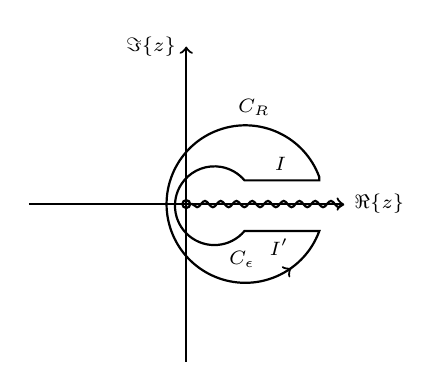
\begin{tikzpicture}
    \begin{scope}[thick,font=\scriptsize,decoration={markings,mark=at position 0.5 with {\arrow{>}}}]
    % Axes:
    % Are simply drawn using line with the `->` option to make them arrows:
    % The main labels of the axes can be places using `node`s:
    \draw [->] (-2,0) -- (2,0) node [right]  {$\Re\{z\}$};
    \draw [->] (0,-2) -- (0,2) node [left] {$\Im\{z\}$};

    % Draw contour
    \draw[postaction={decorate}] (0.75,0) ++(20:1cm) arc (20:340:1cm) -- ++(180:0.95) arc (320:40:0.5cm) -- ++(0:0.95cm) -- cycle;

    \draw (0,0) +(-45:1cm) node {$C_\epsilon$};
    \draw (0,0) +(23:1.3cm) node {$I$};
    \draw (0,0) +(-25:1.3cm) node {$I'$};
    \draw (0,0) +(55:1.5cm) node {$C_R$};

    \draw [decorate,decoration={snake,amplitude=.4mm,segment length=2mm}] (2,0) -- (0,0) node [draw=black, circle, fill=none, inner sep=1pt, pos=1, label] {};
    
    \end{scope}
	\end{tikzpicture}
	\caption{The contour $C = C_R \cup I \cup C_\epsilon \cup I'$, constructed to imitate $C_R$ in the absence of the branch cut along the positive $\mathbb{R}$ axis.}
	\label{fig:r_integration_branch_cut_example}
\end{figure}

\subsection{Closing Contours}
\index{contours}\index{real integrals}

We often complete an $\mathbb{R}$ integral by closing the contour at large $z$. We need to have a bounded integral at large $z$.

\begin{example}{$I = \int_{-\infty}^{\infty} \frac{x\sin{\pi x}}{1 + x^2}\, dx $}
	Let $f(z) = \frac{z\sin{\pi z}}{1+z^2} = \frac{z}{1+z^2} \frac{e^{i\pi z} - e^{-i\pi z}}{2i}$. We want to close this in the upper or lower half-plane, but if $z = R(1 + i\epsilon)$ then:

	\begin{align*}
		e^{i\pi z} &= e^{i\pi R} \cdot e^{-\pi R \epsilon} &\to 0 \text{ as } R\to\infty \\
		e^{-i\pi z} &= e^{-i\pi R} \cdot e^{\pi R \epsilon} &\to \infty \text{ as } R\to\infty
	\end{align*}

	However we can split $f$:

	\[
		f(z) = f_+ (z) + f_- (z) = \underbrace{\frac{ze^{i\pi z}}{2i(1+z^2)}}_\text{convergent on upper half-plane} - \underbrace{\frac{ze^{-i\pi z}}{2i(1+z^2)}}_\text{convergent on lower half-plane}
	\]

	We can thus consider two semi-circular contours $C_\pm$ in the upper/lower half-planes. Note, $C_-$ is traversed clockwise. So

	\[ I = \oint_{C_+} f_+ (z) dz + \oint_{C_-} f_- (z) dz \]

	Both $f_\pm$ have poles at $\pm i$, however $\mp i$ lie outside the contour for $C_\pm$ respectively. Hence:

	\begin{align*}
		Res[f_\pm, \pm i] &= \lim_{z\to\pm i} (z\mp i) f_\pm (z) \\
		&= \lim_{z\to\pm i} \frac{\pm ze^{\pm i \pi z}}{2i(z\pm i)} \\
		&= \frac{ie^{-\pi}}{2i(\pm2i)} \\
		&= \frac{ie^{-\pi}}{\mp 4}
	\end{align*}

	So 

	\begin{align*}
		I &= 2\pi i \left\{ Res[f_+, i] - Res[f_-, -i] \right\} \\
		&= 2\pi i \left\{\frac{ie^{-\pi}}{4} - \frac{ie^{-\pi}}{-4}\right\} \\
		&= \pi e^{-\pi}
	\end{align*}
\end{example}

\section{Summation of Series}
\index{series}

\subsection{The Riemann zeta function}
\index{Riemann zeta function}

Riemann and Euler considered the infinite series

\begin{equation}\label{eq:riemann_zeta}
\zeta(s) = \sum_{n=1}^\infty \frac{1}{n^s}
\end{equation}

This resembles summing residues of poles at $z=n$. We want to construct a meromorphic function with the same poles and residues as the infnite series. Note that we require an infinite number of poles, and recall that trigonometric functions have infinite zeros, providing a good starting point. Now consider:

\[ \frac{1}{\sin{\pi z}} \]

This function has simple poles at $z=n$. We have 

\[ \sin{\pi z} = \sin{n\pi} + \pi\cos{n\pi}(z-n) + ... \]

Given that $\cos{n\pi} = (-1)^n$, the sign of poles of $\sin{nz}$ swaps for even and odd $n$. To avoid this, multiply by $\pi \cos{\pi z}$:

\begin{align*}
h(z) &= \frac{\pi\cos{\pi z}}{\sin{\pi z}} \\
&= \frac{\pi\cos{\pi n} + \mathcal{O}(z-n)^2}{\pi\cos{\pi n} (z-n) + \dots} \\
&= \frac{1}{z-n} + \mathcal{O}(z-n)
\end{align*}

So $h(z) = \pi\cot{\pi z}$ is a `pole-maker'. Combining this with the $\frac{1}{z^s}$ part gives us:

\[ f(z) = \frac{\pi\cot{\pi n}}{z^s} \]

This reproduces the infinite series for $z = n$, but with a pole at $z=0$. Now we need to consider a contour integral of $f$, so we define $C_R = \left\{Re^{i\theta}\right\}: \theta \in [0,2\pi)$. Note that we can only use this contour in the absence of branch cuts for integer values of $s$. In this case, we are interested in $s=4$ and there are no branch cuts. We know how to integrate the $\frac{1}{z^s}$ component, but we need to examine the $\pi\cot{\pi z}$ part:

\begin{align*}
|\cot{\pi z}| &= \left|\frac{e^{i\pi z} + e^{-i\pi z}}{e^{i\pi z} - e^{-i\pi z}}\right| \\
&= \left|\frac{e^{2i\pi z} + 1}{e^{-2i\pi z} - 1}\right| \\
&\to 1 \text{ as } R \to\infty
\end{align*}

However, continuous variation of $R$ causes us to hit poles, so we take the discrete sequence $R=N+\frac{1}{2}$. So:

\[ \left|f(z)\right| = \frac{\pi | \cot{\pi z} |}{|z|^5} \to 0 \text{ as } N \to \infty \]

This implies $\oint_{C_{R,N}} f(z)\, dz \to 0$ as $N\to\infty$, so $\sum_i Res[f,z_i] = 0$.

Now consider $s=4$:

\[ \zeta(4) = \sum_{n=1}^\infty \frac{1}{n^4} \]

Our pole-maker function provides two copies of this infinite series, along the positive and negative real axes. We see $\frac{1}{(-n)^4} = \frac{1}{n^4}$ so $n\in \mathbb{Z}^-$ is equivalent to $n\in \mathbb{Z}^+$. Accounting for the 5th order pole at zero, we have:

\[ 2\zeta(4) + Res[f,0] = 0 \]

So in order to evaluate $\zeta(4)$, we need to find the residue. As this is not a simple pole, we will Taylor expand and use Equation \ref{eq:epsilon}:

\begin{align*}
	f(z) &= \frac{\pi \cot{\pi z}}{z^4} \\
	&= \frac{1}{z^4} \frac{\pi \left(1 - \frac{(\pi z)^2}{2!} + \frac{(\pi z)^4}{4!} + \mathcal{O}(z^6)\right)}{\pi z - \frac{(\pi z)^3}{3!} + \frac{(\pi z)^5}{5!} + \mathcal{O}(z^7)} \\
	&= \frac{1}{z^5} \frac{1 - \frac{(\pi z)^2}{2!} + \frac{(\pi z)^4}{4!} + \mathcal{O}(z^6)}{1 - \frac{(\pi z)^2}{3!} + \frac{(\pi z)^4}{5!} + \mathcal{O}(z^6)} \\
	\intertext{Using Equation \ref{eq:epsilon} with $\epsilon = \frac{(\pi z)^2}{3!} - \frac{(\pi z)^4}{5!}$:} \\
	&= \frac{1}{z^5}\left(1 - \frac{(\pi z)^2}{2!} + \frac{(\pi z)^4}{4!} + \mathcal{O}(z^6)\right)\left(1 + \frac{(\pi z)^2}{3!} - \frac{(\pi z)^4}{5!} + \frac{(\pi z)^4}{(3!)^2} + \mathcal{O}(z^6)\right) \\
	&= \frac{1}{z^5}\left(1 - \frac{(\pi z)^2}{2!} + \frac{(\pi z)^2}{3!} - \frac{(\pi z)^4}{5!} + \frac{(\pi z)^4}{(3!)^2} + \frac{(\pi z)^4}{4!} + \mathcal{O}(z^6)\right)
\end{align*}

So 

\begin{align*}
	Res[f,0] &= \pi^4 \left[\frac{1}{24} - \frac{1}{120} + \frac{1}{36} - \frac{1}{12}\right] \\
	&= -\frac{\pi^4}{45}
\end{align*}

\subsection{Other series}
\index{series}

Consider $S = \sum_{n=1}^\infty \frac{(-1)^n}{n^2}$. Here, we desire the alternating sign characteristic of $\sin{}$, so we don't introduce the $\pi\cos{\pi z}$ part:

\[ f(z) = \frac{\pi}{z^2\sin{\pi z}} \]

We see $\frac{(-1)^{-n}}{(-n)^2} = \frac{(-1)^n}{n^2}$, so again we have two copies of the series plus the pole at zero:

\[ 2S + Res[f,0] = 0 \]

Taylor expanding:

\begin{align*}
	f(z) &= \frac{\pi}{z^2} \frac{1}{\pi z - \frac{(\pi z)^3}{3!} + \mathcal{O}(z^5)} \\
	&= \frac{1}{z^3} \frac{1}{1 - \frac{(\pi z)^2}{3!} + \mathcal{O}(z^4)} \\
	\intertext{Using Equation \ref{eq:epsilon} with $\epsilon = \frac{(\pi z)^2}{3!}$:} \\
	&= \frac{1}{z^3}\left(1 + \frac{(\pi z)^2}{3!} + \mathcal{O}(z^4)\right)
\end{align*}

So $Res[f,0] = \frac{\pi^2}{6}$ and $S = -\frac{\pi^2}{12}$. 

Finally, we will consider the case that a series is not symmetric around the origin. Consider 

\[ f(z) = \frac{\pi\cot{\pi z}}{(z-a)(z+2)} \]

In this case, poles at $z = -n$ are not equal to poles at $z = n$. Instead, consider $m = -n-3$. We see:

\[ (m+1)(m+2) = (-n-3+1)(-n-3+2) = (n+1)(n+2) \]

We now have all poles equated, apart from those at $z=-1, -2$. Hence:

\[ 2S + Res[f,-1] + Res[f,-2] = 0 \]

The pole-maker function has poles at integer $z$ (by construction), so both poles are double poles. In order to evaluate these residues, we will first expand $\pi \cot{\pi z}$ around $z = a$:

\begin{align*}
	\pi \cot{\pi z} &= \frac{\pi\left(1 - \frac{\pi^2(z-a)^2}{2!} + \mathcal{O}(z-a)^4\right)}{\pi (z-a) - \frac{\pi^3 (z-a)^3}{3!} + \mathcal{O}(z-a)^5} \\
	&= \frac{1}{z-a}\frac{\left(1 - \frac{\pi^2(z-a)^2}{2!} + \mathcal{O}(z-a)^4\right)}{1 - \frac{\pi^2 (z-a)^2}{3!} + \mathcal{O}(z-a)^4} \\
	\intertext{Using Equation \ref{eq:epsilon} with $\epsilon=\frac{\pi^2 (z-a)^2}{3!}$:} \\
	&= \frac{1}{z-a}\left(1 - \frac{\pi^2(z-a)^2}{2!} + \mathcal{O}(z-a)^4\right)\left(1 + \frac{\pi^2 (z-a)^2}{3!} + \mathcal{O}(z-a)^4\right) \\
	&= \frac{1}{z-a} + \mathcal{O}(z-a)
\end{align*}

\begin{enumerate}[label={$z_0 =-\arabic*$:}]
	\item{
		We want to find the coefficient of the $\frac{1}{z+1}$ term of $f(z) = \frac{\pi\cot{\pi z}}{(z+1)(z+2)}$ where (see Section \ref{sec:evaluating_poles}). We first need to express $\frac{1}{z+2}$ as an expansion in $(z+1)$ (i.e. around $z=-1$) using Equation \ref{eq:epsilon}:

		\begin{align*}
			\frac{1}{z+2} &= \frac{1}{1+(z+1)} \\
			&= 1 - (z+1) + \mathcal{O}(z+1)^2
		\end{align*}

		We can now assemble $f(z)$:

		\begin{align*} 
			f(z) &= \frac{1}{z+1}\cdot\left(\frac{1}{z+1} + \mathcal{O}(z+1)\right)\cdot\left(1 - (z+1) + \mathcal{O}(z+1)^2\right)\\
			&= \frac{1}{(z+1)^2}\left(1-(z+1) + \mathcal{O}(z+1)^2\right)
		 \end{align*}

		 So $Res[f,-1] = -1$.
	}
	\item{
		Similarly:

		\begin{align*}
			\frac{1}{z+1} &= \frac{1}{-1+(z+2)} \\
			&= -\frac{1}{1-(z+2)} \\
			&= -(1 + (z+2) + \mathcal{O}(z+2)^2)
		\end{align*}

		So:

		\begin{align*} 
			f(z) &= \frac{1}{z+2}\cdot\left(\frac{1}{z+2} + \mathcal{O}(z+2)\right)\cdot-\left(1 + (z+2) + \mathcal{O}(z+2)^2\right)\\
			&= -\frac{1}{(z+2)^2}\left(1+(z+2) + \mathcal{O}(z+2)^2\right)
		 \end{align*}

		 So $Res[f,-2] = -1$.
	}

	Hence we have $2S-1-1=0$, giving $S=1$.
\end{enumerate}

\newpage
\printindex
\end{document}